\chapter{Arquitectura}
\label{chap:arquitectura}

\drop{E}{}ste capítulo analiza en detalle, mediante un enfoque top-down, la arquitectura diseñada para dar soporte al sistema propuesto en este proyecto. Se discutirá la funcionalidad de cada módulo perteneciente a la arquitectura, se explicará cómo están conectados y cómo fluye la información entre ellos hasta obtener el resultado final. 

\section{Visión general de la arquitectura}
\label{sec:visiongeneral}

La arquitectura diseñada (ver Figura~\ref{fig:arquitectura}) es una arquitectura basada en módulos que contribuye a simplificar significativamente el desarrollo del sistema.

\begin{figure}[!h]
\begin{center}
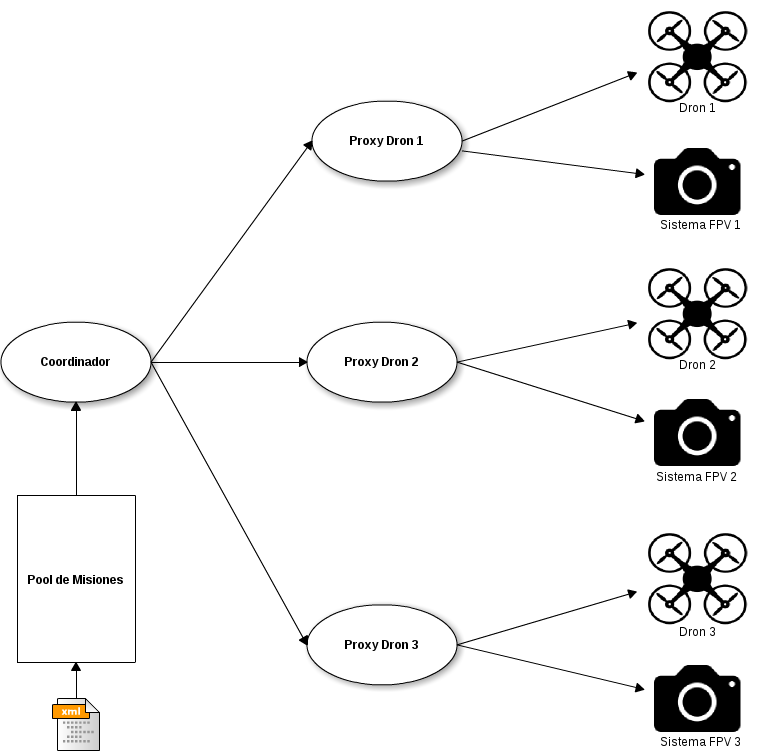
\includegraphics[width=0.63\textwidth]{/arquitectura.png}
\caption[Arquitectura del sistema]{Arquitectura del sistema}
\label{fig:arquitectura}
\end{center}
\end{figure}

Cada módulo representa una clase en la que se definen las propiedades y el comportamiento mediante atributos y funciones. Estas clases son instanciadas en objetos, que se corresponden tanto con objetos reales como con objetos internos del sistema, en los que se realiza la lectura de estas definiciones.

Como se observa, la arquitectura se descompone en cuatro elementos que de forma resumida realizan lo siguiente:
\begin{itemize}
\item \textbf{Coordinador}: realiza una lectura del \textit{Pool de misiones} ordenándolo por prioridad, se encarga de crear instancias del objeto \textit{ProxyDrone}, asignar «waypoints» a vehículos desocupados y ordenar el aterrizaje cuando el \textit{Pool de misiones} este vacío.
\item \textbf{Proxy Dron}: es el responsable a la hora de realizar las operaciones que conciernen al vehículo, como el despegue o la subida de misiones, y de gestionar la conexión con los dispositivos finales, como el \textit{dron} o el \textit{sistema \acs{FPV}}.
\item \textbf{Dron}: Crea una simulación de un vehículo aéreo no tripulado en una localización determinada.
\item \textbf{Sistema FPV}: Captura imágenes en vivo, las analiza y muestra en pantalla los resultados.
\end{itemize} 

En el sistema la información fluye a través de los módulos (ver Figura~\ref{fig:diagflujo}), transformándose hasta alcanzar el resultado final. Esto es, los vehículos aéreos se desplazan de manera coordinada a diversas localizaciones y a su vez retransmiten imágenes, que son analizadas para contribuir a mejorar los tiempos de respuesta en situaciones de emergencia.

\begin{figure}[!h]
\begin{center}
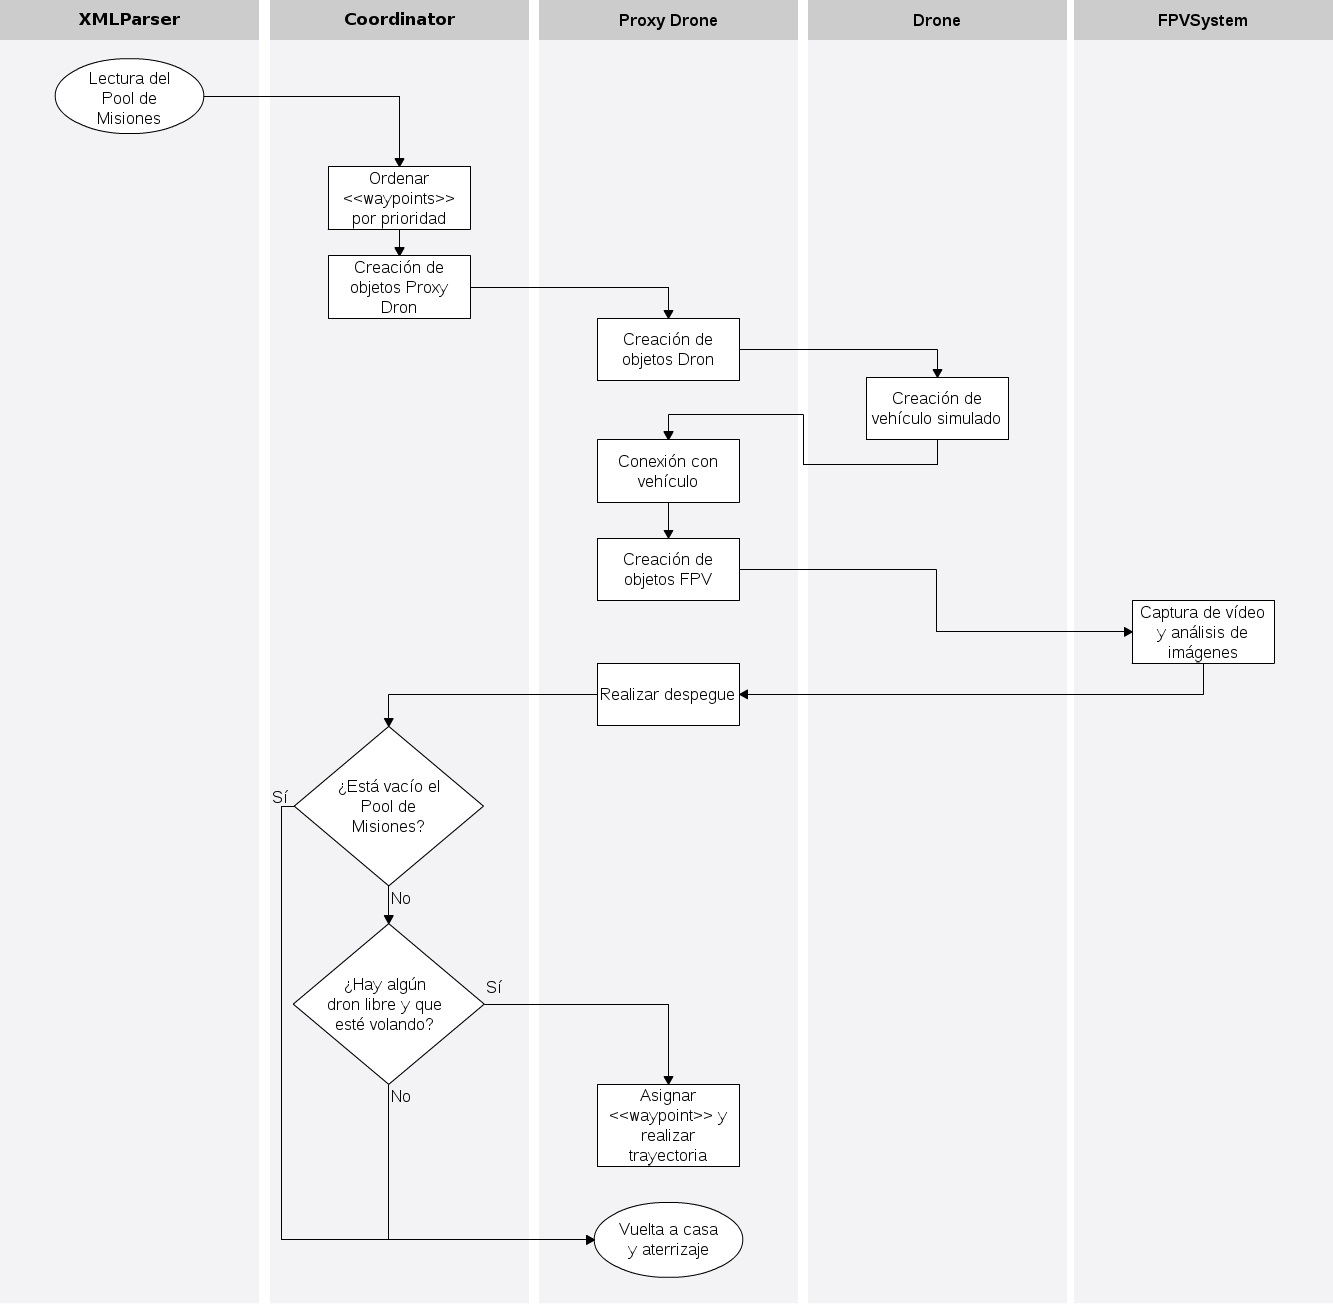
\includegraphics[width=0.8\textwidth]{/Flowchart.png}
\caption[Diagrama de flujo del sistema]{Diagrama de flujo del sistema}
\label{fig:diagflujo}
\end{center}
\end{figure}

\subsection{Coordinador}
\label{sec:coordinador}

El sistema comienza con una llamada a la clase \textbf{\textit{Coordinador}}, la cual cuenta con tres argumentos que son parametrizables al realizar su invocación por consola. Estos atributos parametrizables son los siguientes:
\begin{itemize}
\item \textbf{numVehicles}: se refiere al número de vehículos que participarán en las misiones y capturarán imágenes en directo del vuelo. Si se omite, el valor por defecto es 1 vehículo.
\item \textbf{secondWait}: afecta al número de segundos que el vehículo permanecerá parado sobre un «waypoint» para captar imágenes relevantes de esa localización durante ese tiempo. Si se omite, el valor por defecto es de 10 segundos.
\item \textbf{secondsPerPhoto}: referido al número de segundos que deben transcurrir para tomar una fotografía. Por ejemplo, si el valor es de 5 segundos, el sistema realizará una fotografía cada 5 segundos. Si se omite, el valor por defecto es de 10 segundos.
\end{itemize} 

Un ejemplo de cómo realizar la llamada a \textit{Coordinador} puede ser:

\begin{listing}[
  float=h!,
  language = bash,
  caption  = {Ejemplo de llamada a \textit{Coordinador}},
  label    = code:coordinador]
$ python coordinator.py --vehicles 2 --secondWait 15 --secondsPerPhoto 7
\end{listing}

Este módulo está compuesto por atributos y métodos (ver Figura~\ref{fig:diagclasescoord}) necesarios para llevar a cabo la \textbf{coordinación de los drones}.

\begin{figure}[!h]
\begin{center}
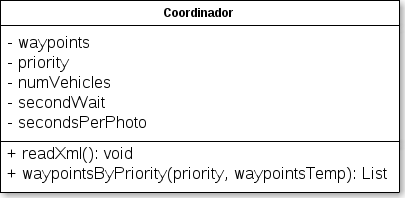
\includegraphics[width=0.8\textwidth]{/clases_coordinador.png}
\caption[Diagrama de clases del \textit{Coordinador}]{Diagrama de clases del \textit{Coordinador}}
\label{fig:diagclasescoord}
\end{center}
\end{figure}

El \textit{Coordinador} es el responsable de \textbf{leer los archivos XML} (ver Listado~\ref{code:archivoxml}) que contiene la información acerca de los puntos de interés a los que los drones deben acudir: \textbf{longitud}, \textbf{latitud}, \textbf{altura} a la que el dron debe volar en dicha posición y la \textbf{prioridad} de que el \acs{UAV} vuele hasta esa localización.

\begin{listing}[
  float=h!,
  language = XML,
  caption  = {Ejemplo de archivo XML que contiene la información de los «waypoints»},
  label    = code:archivoxml]
<?xml version="1.0" ?>
<mission>
	<waypoint>
 		<long>32.8353314496671587</long>
 		<lat>-117.162768244743347</lat>
		<alt>20</alt>
		<priority>2</priority>
	</waypoint>

	<waypoint>
 		<long>32.8353359570248671</long>
 		<lat>-117.161904573440552</lat>
		<alt>40</alt>
		<priority>1</priority>
	</waypoint>

	<waypoint>
 		<long>32.8353359570248671</long>
 		<lat>-117.161904573440552</lat>
		<alt>10</alt>
		<priority>3</priority>
	</waypoint>
</mission>
\end{listing}

Una vez que los archivos XML han sido leídos y los «waypoints» han sido almacenados en una estructura de tipo lista, que denominaremos \textit{Pool de Misiones}, el \textit{Coordinador} debe \textbf{ordenar} esas localizaciones \textbf{por medio del campo prioridad}. La prioridad puede tomar tres valores diferentes: 1, 2 y 3. Siendo 1 la prioridad más elevada y 3 la de menor relevancia. De tal forma que en la lista deben aparecer primero los «waypoints» cuya prioridad sea de 1 y en último lugar los que tengan una prioridad de 3.

Más adelante, se encargará de \textbf{asignar «waypoints»}, hasta vaciar el \textit{Pool de Misiones}, a drones que se hallen en un \textit{estado ocioso} y que se encuentren \textit{en vuelo}. Se considera que un dron está en \textit{estado ocioso} cuando ha terminado de volar a un punto de interés y ha recogido las imágenes especificadas en dicho lugar. 

Por último, cuando el \textit{Pool de Misiones} ha sido vaciado, el \textit{Coordinador} ordena la vuelta a casa y el aterrizaje de cada uno de los drones que se estaban empleando en el proceso.

Es crucial que varios drones puedan efectuar \textbf{a la vez} el vuelo y la captura de vídeo, por lo que es necesario la \textbf{introducción de hilos} que permitan ejecutar, de manera paralela, estas funciones.

\subsection{Proxy Dron}
\label{sec:proxydron}

Tan pronto como se haya realizado la lectura de los archivos XML y se cuente con una lista de «waypoints» ordenados por prioridad, se procede a crear objetos de tipo \textbf{\textit{Proxy Dron}} (ver Figura~\ref{fig:diagclasesproxy}). 
%Para ello, el \textit{Coordinador} hace uso de su atributo \textit{numVehicles}, creando tantos objetos \textit{Proxy Dron} como número de vehículos se haya especificado.

\begin{figure}[!h]
\begin{center}
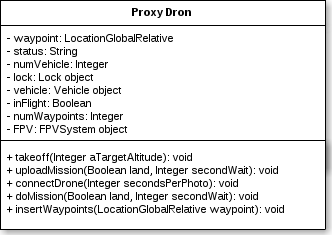
\includegraphics[width=0.8\textwidth]{/clases_proxydron.png}
\caption[Diagrama de clases del \textit{Proxy Dron}]{Diagrama de clases del \textit{Proxy Dron}}
\label{fig:diagclasesproxy}
\end{center}
\end{figure}

El \textit{Proxy Dron} es inicializado pasándole por parámetro el número de vehículo con el que se corresponde dicho objeto. Gracias a esto, el usuario puede obtener \textbf{información del estado del dron}, sabiendo, por ejemplo, si esa información está asociada al \textit{Dron 1} o al \textit{Dron 2}. Es el responsable de llevar a cabo las \textbf{operaciones de vuelo} y de \textbf{administrar la conexión con los dispositivos finales}.

Entre sus competencias se encuentran las que se exponen a continuación:
\begin{itemize}
\item \textbf{Conexión con el dron} y con el \textbf{Sistema FPV}: En el caso de ejecutar una simulación del sistema, se instancia un objeto de tipo \textit{Dron}, que creará un vehículo simulado mediante \acs{SITL} (véase Sección \ref{sec:sitl}). A continuación, se realiza la conexión con el vehículo aéreo, ya sea real o simulado, y por último se crea un objeto \textit{Sistema FPV} para iniciar la grabación y el análisis de imágenes.
\item \textbf{Despegue} del dron: se comprueba que el vehículo cumpla ciertos requisitos antes de armar los motores, como que disponga de una buena señal de \acs{GPS} o que el nivel de la batería sea superior al 50\%, se configura el modo de pilotaje del dron y se procede al despegue a una altura especificada por parámetro. Cuando el despegue ha terminado, el dron se considera \textit{en vuelo}. 
\item \textbf{Inserción de «waypoints»} y \textbf{escritura de misiones}: los «waypoints», que han sido extraidos del archivo XML en el \textit{Coordinador}, son adjudicados a drones que se encuentren en \textit{estado ocioso} y \textit{en vuelo}. La localización de estos puntos debe ser agregada a comandos de misión que puedan ser interpretados por el vehículo. Entre estos comandos se encuentran las órdenes necesarias para: acudir a una localización específica, mantener el vehículo en un punto concreto o realizar la vuelta a casa y el aterrizaje.
\end{itemize}

\subsection{Dron}
\label{sec:dron}

La clase \textbf{\textit{Dron}} (ver Figura~\ref{fig:diagclasesdron}) ofrece la posibilidad de \textbf{simular vehículos aéreos}, en el caso de este proyecto un quadcopter, haciendo uso de la aplicación \acs{SITL} (véase Sección \ref{sec:sitl}).

\begin{figure}[!h]
\begin{center}
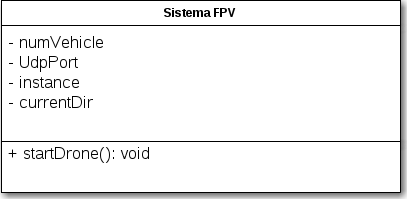
\includegraphics[width=0.8\textwidth]{/clases_dron.png}
\caption[Diagrama de clases del \textit{Dron}]{Diagrama de clases del \textit{Dron}}
\label{fig:diagclasesdron}
\end{center}
\end{figure}

El cometido que tiene este objeto es, dependiendo del número de vehículo que lo instancie, acceder a una carpeta determinada y \textbf{ejecutar el comando} (ver Listado~\ref{code:simulacion}) \textbf{para generar la simulación} del dron, en un puerto UDP concreto, al que posteriormente el sistema se conectará para comunicarse con él.

\begin{listing}[
  float=h!,
  language = bash,
  caption  = {Comando para generar una simulación de un vehículo mediante \acs{SITL}},
  label    = code:simulacion]
$ sim_vehicle.sh -I %d -L prueba --map --out 127.0.0.1:%d --aircraft test
\end{listing}

El comando está formado por unos parámetros que representan lo siguiente:
\begin{itemize}
\item \textbf{-I}: el número de instancia para permitir múltiples copias del simulador funcionando a la vez.
\item \textbf{-L}: ubicación inicial, que es configurada en un archivo de tipo texto denominado \textit{locations.txt}.
\item \textbf{$-$$-$map}: posibilita disponer de una ventana con un mapa, para mostrar el progreso del dron al realizar las misiones.
\item \textbf{$-$$-$out}: dirección en la que se podrá realizar la conexión con el dron. Está formada por una dirección IP y un puerto UDP.
\end{itemize}

\subsection{Sistema FPV}
\label{sec:sistemafpv}

Los objetos de la clase \textbf{\textit{Sistema FPV}} facilitan la captura de imágenes en \acs{FPV} y el análisis de estas.

\begin{figure}[!h]
\begin{center}
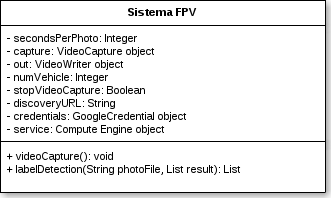
\includegraphics[width=0.8\textwidth]{/clases_fpv.png}
\caption[Diagrama de clases del \textit{Sistema FPV}]{Diagrama de clases del \textit{Sistema FPV}}
\label{fig:diagclasesfpv}
\end{center}
\end{figure}

Las tareas que se desarrollan en esta clase son fundamentalmente tres:
\begin{itemize}
\item \textbf{Grabación de vídeo}: el sistema graba y almacena un vídeo, haciendo uso de OpenCV (véase Sección \ref{sec:opencv}), que facilitará a los equipos de emergencia la visión del terreno, para así, poder tomar unas decisiones mejores y más correctas.
\item Realización de \textbf{cáptura de pantalla}: cada un cierto número de segundos, especificado al realizar la llamada al \textit{Coordinador}, se llevará a cabo una captura de pantalla que será almacenada en el computador y que será utilizada para realizar el análisis.
\item \textbf{Análisis de imágenes}: haciendo uso de Google Cloud Vision \acs{API} (véase Sección \ref{sec:visionapi}) se analizarán las capturas de pantalla realizadas anteriormente. Google Cloud Vision \acs{API}, mediante la detección de etiquetas, detecta amplios conjuntos de categorías y arroja resultados de los elementos que se encuentran dentro de las fotografías. Estos resultados serán imprimidos y mostrados en el vídeo que se está grabando.
\end{itemize}

\clearpage

Para llevar a cabo el análisis de imágenes es necesario realizar una petición HTTP a Google Cloud Vision \acs{API} en la que se especifique el tipo de análisis que se quiere realizar, en este supuesto \textit{Detección de etiquetas}, y el número máximo de resultados que se quieren obtener. Un ejemplo de está petición puede ser la especificada a continuación:

\begin{listing}[
  float=h!,
  language = Python,
  caption  = {Ejemplo de petición a Google Cloud Vision \acs{API} para la detección de etiquetas},
  label    = code:analisis]
with open(photoFile, 'rb') as image:
	image_content = base64.b64encode(image.read())
        service_request = self.service.images().annotate(body = {
        	'requests': [{
                	'image': {
                    		'content': image_content.decode('UTF-8')
                			},
                		'features': [{
                    			'type': 'LABEL_DETECTION',
                    			'maxResults': 5
                		}]
            	}]
        }]
        
		
        response = service_request.execute()
	responseLength = len(response['responses'][0])
\end{listing}


% Local Variables:
%  coding: utf-8
%  mode: latex
%  mode: flyspell
%  ispell-local-dictionary: "castellano8"
% End:
